\documentclass[preprint,12pt]{elsarticle}
\usepackage[T1]{fontenc}
\usepackage{amsmath,amssymb}
\usepackage{graphicx}
\usepackage{booktabs}
\usepackage{url}
\usepackage[expansion=false,protrusion=true]{microtype}
\journal{Journal of Hazardous Materials}
\setlength{\emergencystretch}{2em}

\begin{document}
\begin{frontmatter}

\title{A testing-effort artefact in the most-sensitive aquatic endpoint:
structure-based PFAS screening recovers predictive validity but still cannot
support clearance}

\author[snu]{Jeongyun Kim\fnref{eq}}
\author[cbdri]{Jin Yoo\fnref{eq}}
\author[cbdri]{Ku Kang\corref{cor}}
\ead{bisu9082@gmail.com}
\affiliation[snu]{organization={Department of Chemical and Biological Engineering, Seoul National University},
                  city={Seoul}, country={Republic of Korea}}
\affiliation[cbdri]{organization={CBRN Defense Research Institute}, country={Republic of Korea}}
\cortext[cor]{Corresponding author.}
\fntext[eq]{These authors contributed equally to this work.}

\begin{abstract}
Regulatory hazard screening commonly summarises a substance by the most
sensitive effect concentration reported for it. We show that this convention
makes the response variable a function of how much the substance has been
tested. Across 87 structure-resolved per- and polyfluoroalkyl substances (PFAS)
carrying 4{,}744 freshwater records in the U.S. EPA ECOTOX Knowledgebase, the
protective minimum correlated with the logarithm of record count at Spearman
$\rho=-0.75$ ($p=7\times10^{-17}$); the most-tested quartile sat 4.9
$\log_{10}$ units below the least-tested. Subsampling every substance to equal
depth removed 40--48\% of the association at every depth examined, identifying
that share as an extreme-order-statistic artefact; the remainder is not
attributable to sampling depth alone. The same ordering held across 4{,}757
chemicals. Holding a published random-forest model fixed and changing only the
external target, rank transfer on the same 58 structures rose from
$\rho=+0.09$ to $+0.41$ (difference $+0.32$, 95\% CI $[+0.08,+0.57]$).
Rebuilding training and external sets on an effort-stable acute median restored
external validity and narrowed the prediction interval. Clearance nevertheless
failed: at any threshold matched to the protective endpoint for stringency, no
in-domain PFAS cleared.
\end{abstract}

\begin{keyword}
PFAS \sep aquatic ecotoxicity \sep hazard screening \sep data curation \sep
conformal prediction \sep ECOTOX
\end{keyword}
\end{frontmatter}

\section{Introduction}

Per- and polyfluoroalkyl substances (PFAS) are a structurally diverse class
whose environmental persistence has been argued to be sufficient on its own to
warrant management at the level of the class
\cite{kwiatkowski2020class,cousins2020persistence}, and whose global
distribution and exposure pathways are now extensively documented
\cite{wang2017never,sunderland2019exposure,cousins2022planetary}. The
ecological risk literature for the class has been reviewed in detail
\cite{ankley2021pfasrisk,mccarthy2017pfasecol}, and regulatory programmes have
set out explicit research and action agendas \cite{epa2021roadmap}. Screening
programmes for PFAS nonetheless face an inventory far larger than the measured
record. The U.S. EPA CompTox Chemicals
Dashboard lists tens of thousands of structures
\cite{williams2017comptox,epacomptox2026}, while measured freshwater effect
concentrations exist for a few hundred. Structure-based models are the obvious
way to triage that gap, and quantitative structure--activity relationship (QSAR)
models for aquatic toxicity have a long history
\cite{mazzatorta2005aquatic,nath2023aquatic} with current environmental
applications combining curated descriptors, fingerprints and machine learning
\cite{mansouri2018opera,ms2tox2022,jang2025opqsar}; PFAS-specific models have
followed \cite{sarkar2026pfasqsar}, and multi-endpoint hazard prioritisation
has been proposed as the operational use for such predictions
\cite{kim2026dualthreat}. Best-practice guidance emphasises chemically
independent validation, transparent applicability domains and an explicit
endpoint definition
\cite{tropsha2010best,cherkasov2014qsar,gramatica2007validation}, and the
hazards of reporting internal fit statistics as evidence of predictivity have
been set out repeatedly \cite{golbraikh2002q2}.

Structure-based models are now routinely proposed to fill the data gaps that
block criteria derivation for emerging contaminants
\cite{liang2025datagaps,anand2024grape,khan2019ecotoxqsar}. That a model trained
on conventional organic pollutants transfers poorly to PFAS is established
\cite{cheng2019mlpfas}, and the usual explanation is chemical:
perfluorinated chemistry is absent from the training distribution, so the model
is extrapolating. We report evidence that a second mechanism, independent
of chemistry, contributes substantially to the observed failure.

That mechanism is not unknown qualitatively. The life-cycle assessment
literature has long treated the choice between a lowest-value summary and an
all-data summary as consequential: USEtox builds its effect factor from an
HC50 averaged over all species rather than from the most sensitive species,
and a comparison of the two indicator types showed that the choice of data
source and endpoint by itself reorders the ecotoxicity ranking of chemicals
\cite{saouter2017usetox}. A later data-selection sensitivity analysis of 64
persistent and mobile substances, PFAS among them, reached the same conclusion
for characterisation factors \cite{aggarwal2024cfpm}, and the machine-learning
side has
noted that ``some chemicals have been tested much more often than others'' and
that the resulting target ``rather resembles a probability distribution than a
singular ground truth'' \cite{schur2023adore}. The species sensitivity
distribution literature is the closest antecedent: it has long been established
there that a hazardous concentration estimated from few species is both biased
and imprecise relative to one estimated from many, that the number of species
tested is itself a determinant of the summary, and that the choice of data and
distributional model materially moves the result
\cite{newman2000ssd,aldenberg2000hcunc,wheeler2002ssd,wang2008hc5}. What has
not been done, to our knowledge, is to measure the effect: to quantify the association between a
protective endpoint and testing effort, to separate the part of it that is an
extreme-order-statistic artefact from the part that is not, and to show that the
residual is large enough to invert the apparent external performance of a
published structure-based model. That is what we report.

The mechanism concerns how the response variable is built. Regulatory hazard
assessment is conventionally protective: a substance is summarised by the lowest
effect concentration reported for it, across species, exposure durations and
effect types. The practice is sensible as policy, because the most sensitive
observed effect bounds the hazard. As a statistical construction, however, the
minimum of a sample is an extreme order statistic, and its expected value
decreases as the sample grows. Two substances with identical toxicity will
therefore receive different protective values if one has been tested more often
than the other. Because testing effort varies by orders of magnitude across the
ecotoxicity record --- a handful of records for most substances, thousands for
PFOA and PFOS --- this is not a second-order concern.

If that reasoning is right, three things should follow, and all three are
testable. The protective minimum should correlate with the number of available
records; equalising the number of records should attenuate the correlation; and
a structure-based model, which has no access to testing history, should fail on
the protective minimum while succeeding on an endpoint constructed without the
confound. We test each in turn, using the complete ECOTOX Knowledgebase rather
than a curated subset, and then ask what the corrected picture implies for the
decision the screening programme actually wants to make: whether an untested
PFAS can be set aside as low concern.

\section{Materials and methods}

\subsection{Data source and record selection}

All toxicity data came from the U.S. EPA ECOTOX Knowledgebase ASCII release of
15 September 2026 \cite{olker2022ecotox}, used in full rather than through a
curated derivative such as EnviroTox \cite{connors2019envirotox}, whose
selection rules are appropriate to their own purpose but fix in advance the
record counts whose influence is the object of this study. From 725{,}636 test records we retained tests on aquatic
organisms (\texttt{organism\_habitat} = Water) in freshwater media
(\texttt{media\_type} beginning FW), joined them to 1{,}250{,}612 result
records, and kept results reporting an acute LC50, EC50 or IC50 or a chronic
NOEC, NOEL, LOEC, LOEL or MATC in mass-concentration units convertible to mg/L. Records
carrying an inequality qualifier were identified and excluded from the primary
analysis rather than treated as point observations, because left-censored values
have maximum leverage on the extreme order statistics examined here. Rows identical in test
identifier, endpoint type, reported concentration and unit are duplicates of a
single observation and were collapsed, because testing effort is measured by
counting records and duplicated rows inflate it non-uniformly. This yielded
106{,}095 acute freshwater records for 4{,}757 chemicals, and, for the PFAS
subset defined below, 15{,}991 raw rows reducing to 4{,}744 distinct records
from 2{,}182 tests, carried by 103 CAS registrations that collapse to 87 parent
structures under the standardisation of \S\ref{sec:std}.

PFAS were identified by CAS match to the PFASSTRUCTV6 list of the CompTox
Chemicals Dashboard \cite{epacomptox2026}, the same operational definition used
in the inventory we later deploy against. Structures were resolved from CAS
through PubChem; 4{,}311 of 4{,}757 chemicals (90.6\%) resolved successfully,
and unresolved chemicals were dropped.

\subsection{Endpoint constructions}

Four summaries of the same records were compared. The \emph{minimum} is the
lowest reported value across all acute and chronic strata, which is the
protective convention. The \emph{median} is the median over the same records.
The \emph{acute median} restricts to acute lethality and concentration-response
endpoints before taking the median. The \emph{depth-equalised minimum} draws a
fixed number $k$ of records per substance without replacement and averages the
resulting minima over repeated draws, isolating the effect of sampling depth
while holding the number of records constant by construction. All are expressed
as $y=\log_{10}(T/\mathrm{mg\,L^{-1}})$.

Testing effort was quantified as $\log_{10}$ of the number of usable records for
a substance, and its association with each endpoint was measured by Spearman
correlation. We emphasise that this is a property of the response variable
alone; no model is involved.

\subsection{Structure standardisation}\label{sec:std}

Structures were desalted to the fluorine-bearing fragment where present,
charge-neutralised with the RDKit standardiser and canonicalised
\cite{rdkit,mceachran2018msready}. Desalting to the largest fragment, the more
common convention, misassigns salts whose counterion exceeds the active moiety
in size, and we therefore prefer the fluorinated fragment explicitly.
Substances collapsing to the same parent structure were represented once, and
the standardisation was applied before, not after, the per-substance summaries
were formed: the records of every registration mapping to one parent were
pooled and the endpoint computed once on the pooled set. This matters. Seven of the 103 PFAS CAS
registrations collapse to perfluorooctanesulfonate --- the free acid and six
salts --- and their separately assigned protective values span 7.9 $\log_{10}$
units, from $-6.00$ for the potassium salt to $+1.93$ for the ammonium salt;
treated as distinct substances they enter the analysis seven times, at seven
different effective testing depths. Collapsing them leaves 87
parent structures. PFAS structures and inventory structures were removed from
the broad training set before fitting.

\subsection{Model, validation and conformal intervals}

The representation was a 2{,}048-bit ECFP4 fingerprint (Morgan radius 2)
\cite{rogers2010ecfp} and the learner a random-forest regressor with 300 trees,
$\texttt{max\_features}=\sqrt{p}$ and seed 20260620
\cite{breiman2001random,sklearn}; these are the settings of the published
analysis we re-examine, held fixed so that differences are attributable to the
endpoint and not to tuning. Broad performance used five repeats of shuffled
five-fold cross-validation over structure-locked rows, with 160 trees per fold. External validation
fitted the full broad model once and evaluated it on the PFAS set, with
substance-level bootstrap confidence intervals on Spearman $\rho$ (4{,}000
resamples, except the fixed-model comparison of SI Table~S7, which used
3{,}000).

Normalised split-conformal intervals used the nonconformity score
\begin{equation}
s_i=\frac{|y_i-\hat y_i|}{\sigma_i+\beta},
\end{equation}
with $\sigma_i$ the standard deviation across forest trees and $\beta$ the
median calibration $\sigma$ plus $10^{-6}$, and the finite-sample order
statistic $\lceil(n+1)(1-\alpha)\rceil$
\cite{vovk2005algorithmic,shafer2008tutorial,lei2018distfree}. Normalising the
residual by a model-derived difficulty estimate, rather than using the bare
absolute residual, is the standard device for obtaining substance-specific
rather than constant-width intervals
\cite{papadopoulos2011cpknn,cortesciriano2019deepconf}, and the procedure has
an established record in {QSAR} applications
\cite{norinder2014conformal,angelopoulos2023gentle}. Marginal calibration used a random
80/20 split of the broad set, evaluated on the PFAS set. PFAS-conditional
calibration held the broad model fixed and split the PFAS set into disjoint
calibration and test halves. Both were repeated 40 times and means reported. The distinction matters
because the split-conformal guarantee is marginal over an exchangeable
calibration and test pair; conditional validity on a subpopulation is a strictly
stronger requirement that marginal calibration does not deliver
\cite{vovk2012conditional}.

\subsection{Applicability domain and clearance}

The applicability domain was the mean Euclidean distance in ECFP4 space to the
five nearest training structures, thresholded at the 95th percentile of
training leave-self-out distances; this is the $k$-nearest-neighbour
formulation among the standard families of domain definition
\cite{sahigara2012ad,sahigara2013knnad}. The choice of metric is not neutral
for binary fingerprints, since Euclidean distance counts shared absences as
evidence of similarity while Tanimoto does not \cite{bajusz2015tanimoto}; we
report both and the resulting domain memberships in SI \S S10. Conformal
intervals have themselves been proposed as a domain criterion
\cite{norinder2016cpad}, and out-of-distribution alerting serves the same
function in open-set classification settings
\cite{kang2026openset,kim2026driftrobust}. A structure was \emph{cleared} when the lower
bound of its 90\% interval exceeded the hazard threshold. Because the endpoint
constructions differ in protectiveness, clearance was evaluated across a
continuum of thresholds rather than at a single value, and reported at three
reference points: 0.1 mg/L, the value used with the protective minimum; 1 mg/L,
the Globally Harmonised System acute aquatic Category 1 boundary; and a
stringency-matched value obtained by shifting 0.1 mg/L by the measured offset
between the two endpoints.

\subsection{Subclass assignment}

PFAS were assigned to structure categories following the OECD (2021) definition
and the 2018 OECD/UNEP structure series
\cite{oecd2021pfas,buck2011terminology}, the same categorisation logic that
underpins regulatory category and read-across approaches for the class
\cite{patlewicz2019category}.
The definitional gate requires at least one fully fluorinated, saturated methyl
or methylene carbon with no hydrogen, chlorine, bromine or iodine attached;
methine ($>$CF--) and unsaturated ($=$CF$_2$) carbons do not satisfy it.
Categories were then assigned by parsing the molecule as
C$_n$F$_{2n+1}$--X--R, with head-group identity taking precedence over
incidental fluorination, so that a perfluoroalkyl ether acid is recorded as an
ether acid rather than as a chain compound.

\section{Results and discussion}

\subsection{The protective minimum tracks how much a substance has been tested}

Across the 87 parent structures with freshwater records, the protective minimum
correlated with the logarithm of the number of available records at
$\rho=-0.749$ ($p=7\times10^{-17}$; Figure~\ref{fig:effort}a). The same
correlation computed on the number of distinct tests rather than records is
$\rho=-0.703$. The gradient is not subtle. Binned by record-count quartile, the
median protective value falls monotonically from $+1.16$ $\log_{10}$ mg/L in the
least-tested quartile through $-0.52$ and $-2.00$ to $-3.76$ in the most-tested,
a difference of 4.9 $\log_{10}$ units (Mann--Whitney $p=1\times10^{-7}$); the
comparison between substances with three or fewer records and those with at
least a hundred is 6.3 units. Either span is larger than the entire range the
modelling literature attempts to predict.

The same substances illustrate the mechanism individually. Per\-fluoro\-octane\-sulfonic acid carries 1{,}548 distinct freshwater records from 690 tests and
perfluorooctanoic acid 1{,}232 from 679; the minimum of each is $-6.00$. Under
the protective convention each is summarised by the lowest value in its own
large sample. These extreme values are not data-entry errors --- they are
genuine entries in a public, curated database --- but they are the minima of
very large draws from very wide distributions, and a substance tested twice
cannot produce a comparable minimum however toxic it is.

\begin{figure*}[t]
\centering
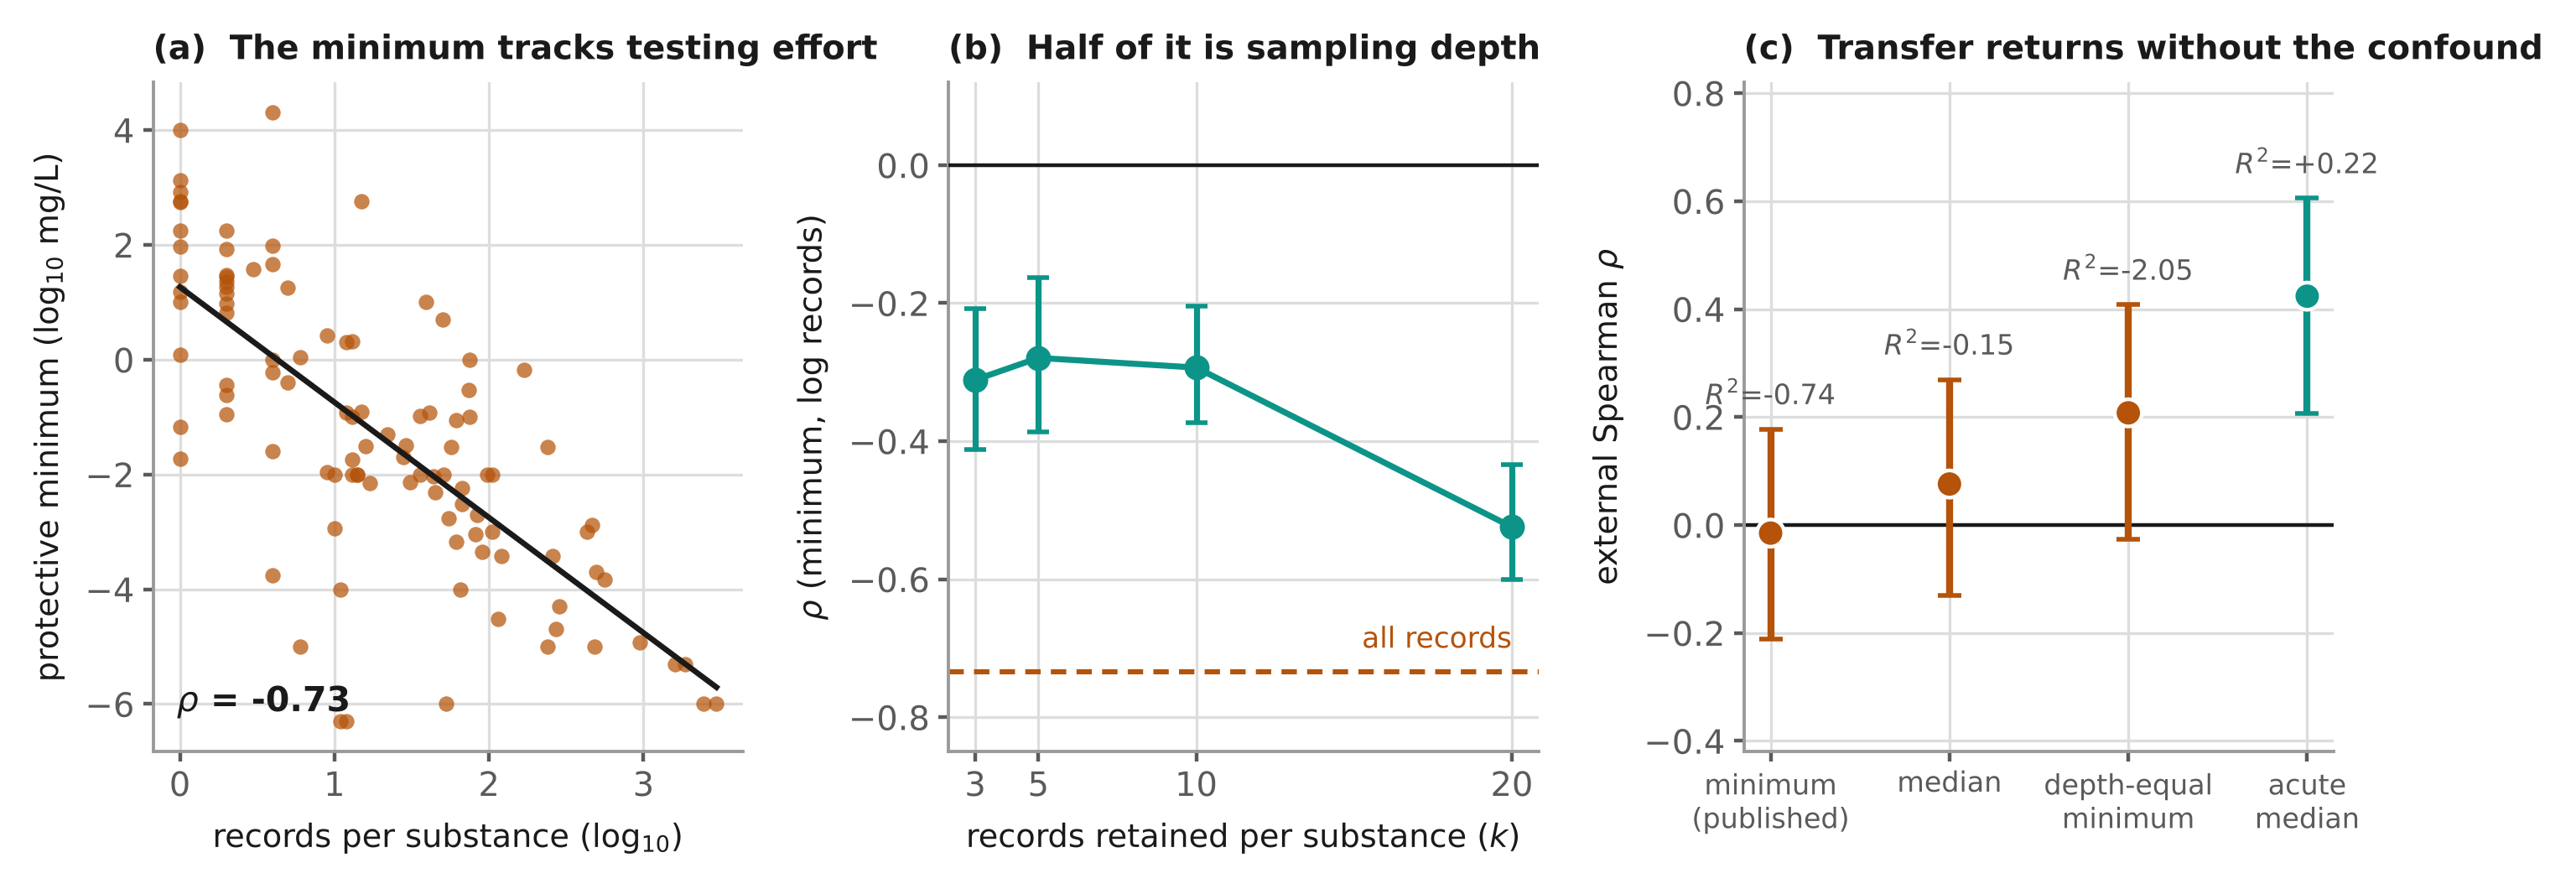
\includegraphics[width=\linewidth]{fig_01_effort.png}
\caption{The protective endpoint is confounded with testing effort. (a) Protective
minimum against the number of de-duplicated freshwater records per PFAS parent
structure ($n=87$). (b) Spearman correlation between the minimum and the record
count after subsampling every eligible substance to depth $k$ (teal), against
the same substances using all of their records (grey); the gap between the two
lines is the depth effect, and the dotted line is the value over all 87
substances. Bars are standard deviations over 400 draws. (c) External rank
transfer of a fixed broad non-PFAS model on the 58 parent structures common to
both endpoints, with 95\% bootstrap intervals and the paired difference
annotated.}
\label{fig:effort}
\end{figure*}

\subsection{Sampling depth accounts for 40--48\% of the association}

Correlation between effort and the protective value admits explanations that
are not mutually exclusive. Substances of greater concern attract more testing,
which would make the association causal in the reverse direction; more-tested
substances also accumulate a wider range of species, durations and effect types,
so their records are drawn from a more dispersed distribution; and the minimum
of a larger sample is lower by construction. Subsampling isolates the last of
these. Because a substance is eligible for depth $k$ only if it has at least $k$
records, the comparison must be made against the same substances at full depth
rather than against the whole set, or the change in sample is read as an effect
of depth. Against that baseline the depth effect was $0.36$, $0.31$, $0.30$ and
$0.30$ at $k=3,5,10$ and $20$ (Figure~\ref{fig:effort}b), i.e.\ 40--48\% of the
full-sample association and stable in $k$; the apparent anomaly at $k=20$ in a
whole-set comparison is an artefact of the shifting denominator.

We do not attribute the residual to reverse causation. That the measured
toxicity of a PFAS varies substantially across studies, species and designs is
itself well documented, and has been quantified by meta-regression across the
class \cite{shabaka2026metareg}. Within-substance
dispersion itself rises steeply with effort in these data (SI \S S3), and
subsampling draws from each substance's own pool, so it preserves that
substance's dispersion and assay mix by construction and cannot remove that
channel. The residual $\rho\approx-0.34$ is therefore not attributable to
sampling depth alone, and reverse causation and effort-dependent assay breadth
are not separable in this design.

The effect is not peculiar to PFAS. Over all 4{,}757 chemicals with freshwater
acute data, the acute minimum carried $\rho=-0.46$ against record count while
the acute median carried $\rho=-0.16$ --- a threefold difference between two
summaries of identical records. The confound is a property of taking a minimum,
not of the chemical class.

\subsection{Transfer failure follows the confound, not the chemistry}

A structure-based model has no access to a substance's testing history. If the
protective endpoint is partly a measure of that history, the model should fail
on it for reasons unrelated to chemistry. Holding the published broad non-PFAS
model fixed and changing only the external target tests this directly
(Figure~\ref{fig:effort}c). An acute median is defined only for substances
carrying acute records, so the four constructions are not available on identical
substance sets; we therefore report the comparison on the 58 parent structures
common to the protective minimum and the acute median. On those same 58
structures the minimum gave $\rho=+0.086$ (95\% CI $[-0.18,+0.35]$) and the
acute median $\rho=+0.412$ ($[+0.18,+0.60]$); a paired bootstrap on the
difference gives $+0.321$ ($[+0.08,+0.57]$, $p=0.005$). Only the acute median's
interval excludes zero. Across all four constructions on their full available
sets, the ordering of external rank performance is the ordering of freedom from
the effort confound (SI Table~S7).

We lead with rank rather than $R^2$ deliberately. The protective minimum sits
$2.2$ $\log_{10}$ units below the training target's mean, and that constant
accounts for most of its apparent $R^2$ collapse: removing a single intercept
moves the minimum from $R^2=-0.714$ to $+0.011$ and the acute median from
$+0.247$ to $+0.325$. The $R^2$ contrast therefore restates the location shift
that the order-statistic mechanism produces, and is not independent evidence
about predictive structure. The rank contrast is, and it survives the matched
comparison above. Variance compression is also visible and should be reported:
the ratio of predicted to observed standard deviation is $0.34$ on the minimum
against $0.59$ on the acute median.

This also accounts for an observation reported previously without a mechanism.
Restricting to acute endpoints has been noted to improve external rank
correlation, and attributed to heterogeneity in assay availability. The present
analysis identifies what that heterogeneity is: acute-only restriction removes
most of the effort confound, because acute lethality endpoints are reported in a
narrower range and the median is not an extreme order statistic.

\subsection{Consistent rebuilding restores predictive validity}

The comparison above changed the external target while leaving the training
target as published. Rebuilding both consistently on the acute median gave a
broad training set of 3{,}718 structure-locked non-PFAS chemicals, of which
3{,}717 yielded a valid fingerprint and entered the model, and an
external set of 58 structure-locked PFAS. Broad cross-validation improved from
$R^2=0.387\pm0.024$ to $0.443\pm0.029$. External validation improved from
$R^2=-0.580$ to $+0.366$ and from $\rho=-0.071$ to $+0.460$ (95\% CI
$[+0.23,+0.65]$) (Figure~\ref{fig:rebuild}a).

Interval behaviour improved correspondingly, with two qualifications we state
rather than leave to the reader. Marginal calibration, which under-covered PFAS
badly on the protective endpoint (0.659 at nominal 0.90), reached 0.851, and
PFAS-conditional calibration reached 0.897. Both are estimated on 58 and 29
external structures respectively, so their intervals are wide: 95\% CI
$[0.73,0.93]$ for the marginal and $[0.73,0.98]$ for the conditional. Neither
differs significantly from the nominal 0.90, but the design could not have
detected coverage as low as 0.81 either, and these figures should be read as
estimates with a spread of about $\pm0.10$, not as demonstrations of validity
(SI Table~S9). Marginal calibration
moreover splits the broad non-PFAS set and tests on PFAS, so exchangeability
fails by construction and no conformal guarantee applies to it; the conditional
procedure, calibrated and tested within PFAS, is the one with a theoretical
basis, and it is also the one we deploy.

The conditional median 90\% interval narrowed from 10.53 to 4.48 $\log_{10}$
mg/L (2.5th--97.5th percentile over 40 calibration splits $[3.34,5.35]$;
Figure~\ref{fig:rebuild}b), but the greater part of that narrowing is the
target being less dispersed rather than the model being better. On the 58
matched structures the ratio of standard deviations is $1.58/2.67=0.59$, so a
width of about 6.2 units would follow from the change of target alone; the
achieved 4.48 improves on that, and the comparison that carries the practical
meaning is 4.48 against the 2.43 that would be required for the median
in-domain structure to clear at the 1 mg/L decision point (SI \S S6). We therefore do not claim that the interval was halved by
better prediction.

\begin{figure*}[t]
\centering
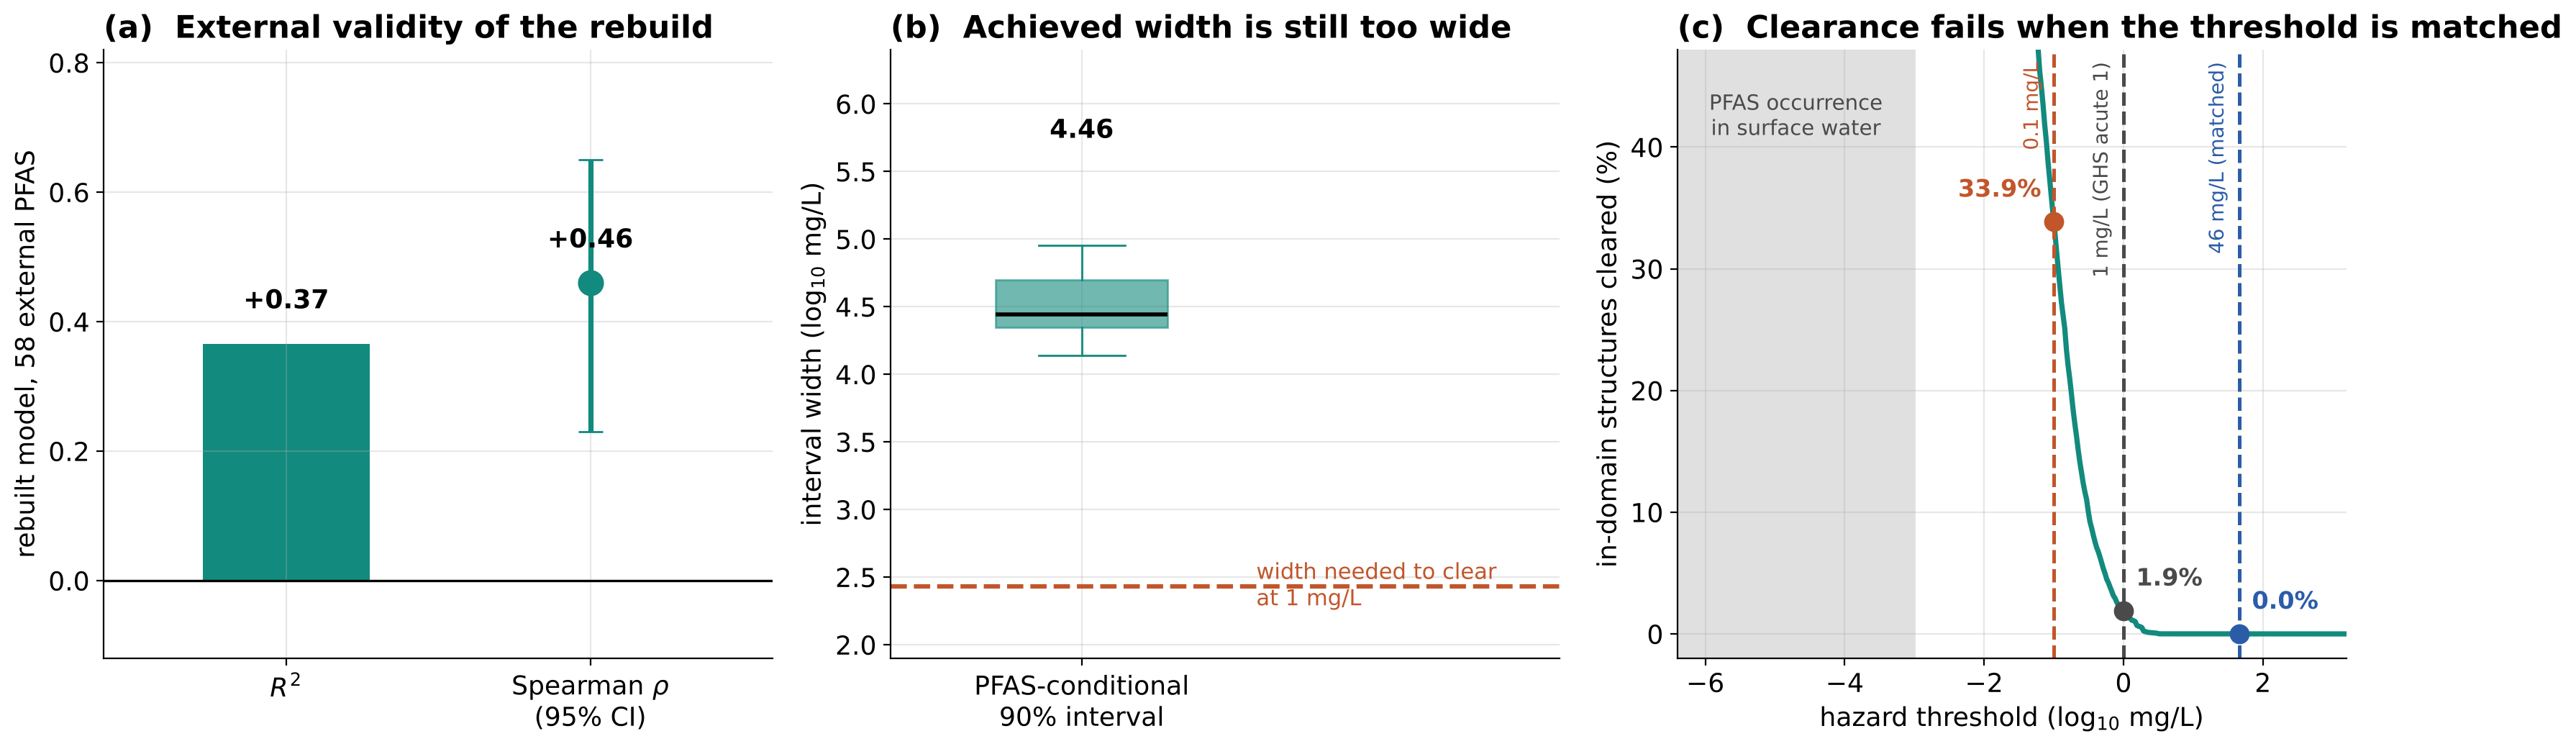
\includegraphics[width=\linewidth]{fig_02_rebuild.png}
\caption{The rebuilt model. (a) External validation on 58 structure-locked
PFAS, with the 95\% bootstrap interval on Spearman $\rho$. (b) PFAS-conditional
90\% interval width over 40 calibration splits, against the width that would be
required for the median in-domain structure to clear at 1 mg/L. (c) Fraction of
in-domain inventory structures cleared as a function of the hazard threshold.
Three reference thresholds are marked: the value used with the protective
endpoint, the GHS acute Category 1 boundary, and one construction of a
stringency-matched value. The shaded band is the concentration range in which
PFAS are reported in surface water; the modelled effect concentrations lie
several orders of magnitude above it, as hazard terms necessarily do.}
\label{fig:rebuild}
\end{figure*}

\subsection{Clearance still fails once the threshold is matched}

Applied to the untested inventory, the rebuilt model placed 16{,}070 of 17{,}619
unique structures inside the applicability domain with a median interval width
of 4.87 $\log_{10}$ units, and cleared 5{,}441 of them (33.9\%) at the 0.1 mg/L
threshold used with the protective endpoint. That number must not be compared
with the zero reported for the protective endpoint, and the reason is
quantitative. On the same 58 structures the acute median lies above the
protective minimum by 2.66 $\log_{10}$ units in the mean and 2.32 in the median,
and 93.1\% of measured PFAS exceed 0.1 mg/L on the acute median against 39.7\%
on the minimum. The threshold means something
different on each endpoint, and holding it fixed while changing the endpoint
relaxes the decision rather than improving it.

Evaluating clearance across thresholds removes the ambiguity
(Figure~\ref{fig:rebuild}c). At the GHS acute aquatic Category 1 boundary of 1
mg/L, 306 structures clear (1.9\%). At a threshold shifted to match the protective
endpoint for stringency, none clear. That threshold is a construction, not a
regulatory object, and it is not unique: the mean paired offset puts it at 46
mg/L, the median offset at 21 mg/L, and matching instead on the fraction of
measured PFAS falling above the cut-off (39.7\% on the minimum) puts it at 41
mg/L. Clearance is zero
at all three, and at every threshold at or above 10 mg/L, so the conclusion does
not depend on which construction is chosen (SI Table~S10). The published
conclusion that no untested PFAS can be cleared therefore
survives, and survives on a model that now has demonstrated external validity
rather than on one that had none.

What changes is the explanation, and the two reference thresholds fail for
different reasons. The obstacle is not that structure-based models cannot
predict PFAS aquatic toxicity; on a properly constructed endpoint they predict
it with $R^2=+0.37$ and a rank correlation whose interval excludes zero. At the
GHS Category 1 boundary the obstacle is uncertainty: the median in-domain
structure would clear with a 90\% interval of 2.43 $\log_{10}$ units against the
4.87 achieved, so halving the interval again would be sufficient. That is a
concrete target, and one the previous framing could not have specified, because
an endpoint confounded with testing effort does not define a stable distance to
any threshold.

At the stringency-matched threshold the obstacle is different and more
fundamental. There the median in-domain structure has a point prediction
\emph{below} the threshold, so the required half-width is negative and no
narrowing of the interval would clear it. At protective stringency the model is
not uncertain about whether these structures are low hazard; it predicts that
most of them are not. Separating these two regimes matters for research
planning, because only the first is addressed by better uncertainty
quantification.

\subsection{Structure classes cannot be resolved at available sample sizes}

A natural next question is whether transfer differs across PFAS structure
classes, since the chemical argument for extrapolation failure is
class-specific, and aquatic potency within the class does vary systematically
with chain length and head group
\cite{conder2008pfca,brendel2018short,gomis2018potency}. We tested this on OECD (2021) categories and report a negative
result with its power requirement, because the point estimates invite
over-reading.

We classify on the acute median, the endpoint this paper endorses: a
class-resolved analysis of the protective minimum would inherit the effort
confound a class at a time. Of the 87 parent structures, the OECD definitional
gate admits 83; the four it excludes are difluoroacetic acid, whose CHF$_2$
carbon is not fully fluorinated, pentafluoroaniline, pentafluorobenzaldehyde and
1,1,2-trichlorotrifluoroethane. Fifty-six of the 83 carry acute records and
enter the comparison, distributed across nine categories, of which six reach
five substances; the two smallest, perfluoroalkyl ether acids and ether others
at three substances each, and perfluoroalkyl phosphorus compounds, which carry
no acute record at all, are reported in SI Table~S11 but not estimated, since a
bootstrap interval on three points is degenerate.

\emph{No category resolves.} Pooled across all classified PFAS the model
transfers at $\rho=+0.41$ (95\% CI $[+0.18,+0.61]$, $n=56$), but every one of
the six estimable categories has an interval covering zero, from
$\rho=-0.44$ for fluorotelomers ($n=9$) to $+0.68$ for the residual
perfluoroalkyl category ($n=7$) (Figure~\ref{fig:subclass}). This is a cleaner
negative result than the one we reported previously on a superseded data
extraction, where a single category appeared to exclude zero; that estimate does
not survive recomputation on the present set, and we note the correction
explicitly. We also tested whether class-level transfer merely tracks class-level
testing effort, which would make the figure a third measurement of the confound
rather than a statement about chemistry: it does not
($\rho=-0.49$, $p=0.33$, between class rank correlation and class mean
$\log_{10}$ record count across the six estimable classes --- negative, and far
from significant on six points).

Power is the binding constraint. At these category sizes, 80\% power at
$\alpha=0.05$ detects only $|\rho|\ge0.71$ to $0.92$. Resolving differential
transfer at a more realistic effect size of $\rho=0.3$ would require
approximately 85 measured substances per category, or 129 with correction for
six comparisons --- roughly 510 to 780 measured PFAS against the 87 parent
structures the public record currently supports. This is the quantity a
programme that wants class-resolved screening would need to measure, and it is
six to nine times what exists. Measuring that many substances at random is not
the only option: where the cost of an experiment dominates, the selection of
which substances to test is itself a design variable, and active or
model-guided selection routinely attains a given accuracy with a fraction of
the measurements required under random sampling
\cite{settles2009active,smith2018less,graff2021molpal,lookman2019active}. We
note it as the obvious route to the sample sizes above rather than as a result
of this study.

\begin{figure}[t]
\centering
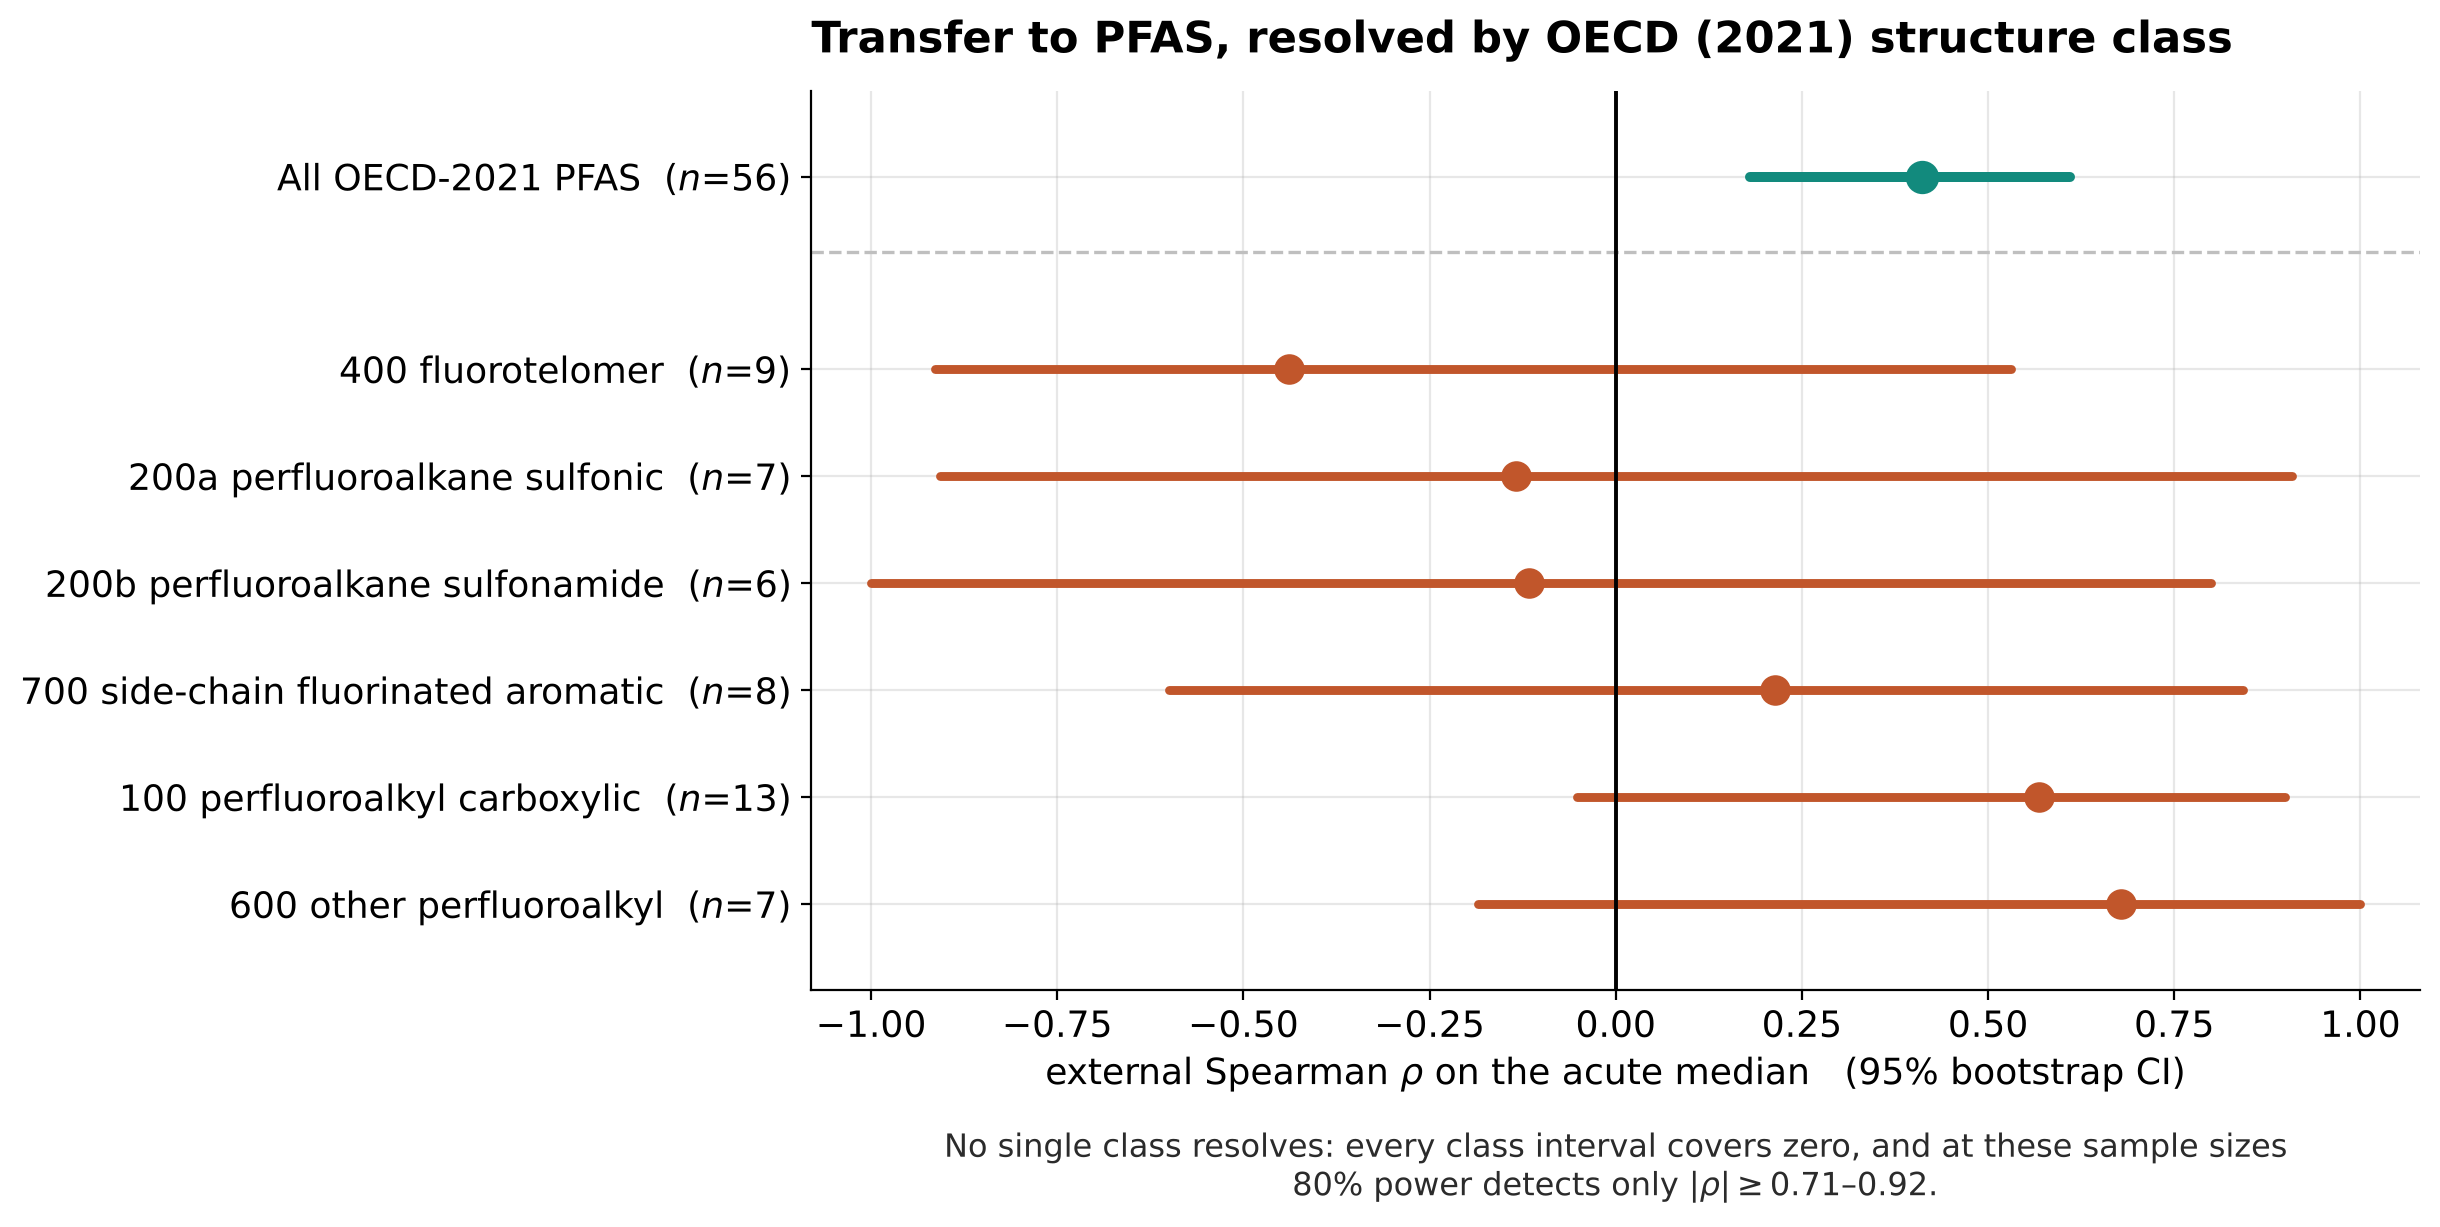
\includegraphics[width=\linewidth]{fig_03_subclass.png}
\caption{External rank correlation by OECD (2021) structure class on the acute
median, with 95\% bootstrap intervals. The pooled estimate excludes zero; no
individual category does. Categories with fewer than five substances are listed
in SI Table~S11 and not estimated.}
\label{fig:subclass}
\end{figure}

\subsection{Implications for screening practice}

Four consequences follow for programmes that build or consume structure-based
hazard screens.

First, the response variable deserves the scrutiny usually reserved for the
model. A protective minimum taken over a heterogeneous record is not a property
of the substance alone, and the degree to which it is not can be measured
directly with the correlation reported here. We would suggest that any
screening study report the association between its endpoint and the number of
underlying records, as a routine diagnostic, in the way applicability domains
and condition-dependence are now routinely reported
\cite{kang2026dbpcarto}.

Second, a model that fails external validation on a protective endpoint has not
thereby been shown to lack chemical validity. The failure is consistent with the
model being unable to predict testing history, which is not a chemical
deficiency. Endpoint construction is not the only lever: on the earlier
extraction of this work, holding the endpoint at the protective minimum and
replacing the binary ECFP4 representation with 165 physicochemical descriptors
also recovered rank transfer, from $\rho=-0.03$ to $+0.42$ (SI Table~S12), and a
ridge baseline outperformed the random forest on the same target (SI
Table~S13). Both tables are from the superseded extraction and we have not
repeated them on the present one, but the direction is clear enough that the
claim must be made in the weaker form. There is a mechanistic reason to expect
representation to matter for this class: much of PFAS bioactivity is mediated
by binding to serum proteins and to nuclear receptors, with potency depending
on chain length and head group in ways a topological fingerprint does not
encode
\cite{cheng2018protein,vandenheuvel2006ppar,wolf2008ppar}. Endpoint and representation therefore both matter.
We report the endpoint comparison because it is the larger of the two on matched
samples, because it is the one a screening programme controls when it defines its
response variable, and because it is inexpensive; we do not claim that
representation is irrelevant.

Third, the confound propagates to the concentrations at which PFAS are actually
regulated, which are far below those modelled here. PFAS occur in surface water
at nanograms to low micrograms per litre; the European environmental quality
standard for perfluorooctanesulfonate in inland surface water is 0.65 ng/L
\cite{eu2013directive} and the United States maximum contaminant level for
perfluorooctanoate and perfluorooctanesulfonate is 4 ng/L \cite{epa2024mcl}, while the effect concentrations modelled
here, and the 0.1 to 1 mg/L decision boundaries applied to them, sit five to
seven orders of magnitude higher. That gap is not an artefact of this study: it
is the standard structure of hazard assessment, in which a predicted no-effect
concentration is an effect concentration divided by an assessment factor, so the
hazard term is necessarily derived at effect concentrations and only then
brought down to the occurrence range. The consequence is that an effort
confound in the effect term is not diluted by that division --- an assessment
factor is a multiplicative constant and leaves a 4.9 $\log_{10}$ unit gradient
intact. A criterion derived at nanograms per litre from a minimum-based hazard
term inherits the whole of it. This is why we regard the diagnostic as
environmentally consequential rather than merely methodological, and it is also
why we do not present the clearance fractions as risk estimates: a clearance
rule that compares a predicted effect concentration directly with a fixed
cut-off, as the screening literature we re-examine does, carries no exposure
term, and the fractions below should be read as a property of that decision
rule.

Fourth, the protective convention is not thereby wrong. It remains the correct
posture for a regulatory decision, because the lowest observed effect does bound
the hazard. What the present results argue is that it is unsuitable as a
\emph{regression target}, and that screening pipelines should model an
effort-stable quantity and apply protectiveness at the decision step rather than
embedding it in the response variable where it cannot be separated from testing
history.

We are deliberate about what that does and does not propose. It is not a
proposal to substitute a median into an existing assessment-factor schedule.
Those schedules are calibrated over a \emph{lowest} value from a specified set
of trophic levels --- ECHA Guidance R.10 assigns a factor of 1000 to the lowest
short-term L(E)C50 across three trophic levels \cite{echa2008r10} --- and no published calibration
exists for a median, so swapping the summary underneath an unchanged factor
would leave the factor undefined. The claim is narrower: when a structure-based
model is fitted in order to \emph{prioritise} untested substances, its
regression target should be effort-stable, and protectiveness should re-enter
when the prioritised substances are carried into an assessment. We also note
what the record-level acute median is not. It is a median over records, not
over species: the ECOTOX extraction used here does not carry a species field, so
a substance tested fifty times in \emph{Daphnia magna} and once in a fish is
summarised by a value that is effectively the \emph{Daphnia} result. The
species-aggregated alternatives --- a geometric mean per species feeding a
species sensitivity distribution, with the HC5 as the summary
\cite{posthuma2019ssd} --- are both
effort-stable and protective, have a mature methodological literature, and are
the natural target for a screening model built on a species-resolved
extraction. We did not evaluate them here because the extraction we re-used
from the study under re-examination does not carry species, and we regard that
comparison as the most useful next step rather than a gap we can close in this
paper.

\subsection{Limitations}

The external PFAS set contains 58 structure-locked substances on the acute
median, smaller than the 87 parent structures available on the protective
endpoint, because restricting to acute endpoints removes the 29 substances whose
records are entirely chronic. This is the
principal limitation and it bounds the precision of every external statistic
reported. Structures resolved for 90.6\% of chemicals; the unresolved remainder
may be non-random with respect to chemical class, which we could not assess.
The acute median remains a mixture over species, exposure duration and effect
type, and is effort-stable rather than effort-free. The clearance analysis
evaluates aquatic effect concentrations only and says nothing about exposure,
persistence or bioaccumulation, which are the properties that in practice drive
PFAS regulatory action; a substance with a high acute LC50 and a decades-long
half-life is not low concern, and no aquatic-toxicity model of any quality would
establish that it was. Finally, the residual association that survives depth
equalisation is not identified: this design cannot separate reverse causation
from effort-dependent assay breadth, and the latter is not removed by
subsampling.

\section{Conclusions}

Summarising a substance by the lowest effect concentration ever reported for it
makes the resulting value depend on how often it has been tested. Across 87
PFAS parent structures the protective minimum correlated with record count at
$\rho=-0.749$, and equalising sampling depth against the eligible-subset
baseline identified 40--48\% of that as an extreme-order-statistic artefact;
across 4{,}757 chemicals the acute minimum carried three times the confound of
the acute median. Because a structure-based model cannot predict testing
history, this confound contributes to the external validation failures reported
for PFAS screening: holding a published model fixed and changing only how the
same records are summarised raised rank transfer on the same 58 parent
structures from $\rho=+0.09$ to $+0.41$, a paired difference of $+0.32$
(95\% CI $[+0.08,+0.57]$, $p=0.005$).

Rebuilding training and external sets consistently on the acute median restored
external validity ($R^2=+0.37$; $\rho=+0.46$, 95\% CI $[+0.23,+0.65]$) and
narrowed the PFAS-conditional interval to 4.48 $\log_{10}$ mg/L, most of that
narrowing being attributable to the less dispersed target rather than to better
prediction. Clearance
nevertheless failed at a stringency-matched threshold, where no in-domain
inventory structure cleared, and at the GHS acute Category 1 boundary, where
1.9\% did. The conclusion that structure-based screening cannot presently clear
untested PFAS therefore stands, but it stands for a reason the earlier framing
did not identify: not that such models cannot predict PFAS aquatic toxicity, but
that a validated model's interval, and at protective stringency its point
prediction, remain on the wrong side of the decision threshold. The practical
recommendation is to model an effort-stable endpoint, report the
endpoint--effort association as a routine diagnostic, and apply protectiveness
at the decision step rather than inside the response variable.

\section*{CRediT authorship contribution statement}
\textbf{Jeongyun Kim:} Methodology, Software, Formal analysis, Writing --
original draft. \textbf{Jin Yoo:} Data curation, Validation, Formal analysis,
Writing -- review \& editing. \textbf{Ku Kang:} Conceptualization, Supervision,
Methodology, Writing -- original draft, Writing -- review \& editing.

\section*{Funding}
This research did not receive any specific grant from funding agencies in the
public, commercial, or not-for-profit sectors.

\section*{Declaration of competing interest}
The authors declare that they have no known competing financial interests or
personal relationships that could have appeared to influence the work reported
in this paper.

\section*{Declaration of generative AI in the writing process}
During the preparation of this work the authors used a large language model to
assist with code development for data extraction and analysis, and with language
editing. The authors reviewed and edited all output and take full
responsibility for the content of the publication.

\section*{Data availability}
All extraction and analysis scripts, the structure-locked tables, and the
inventory-level predictions are openly available at
\url{https://github.com/bisu9082/pfas-clearance-validation}, tagged as release
\texttt{v3.2}. Every number reported in this paper and its Supporting
Information, and every figure including the graphical abstract, is regenerated
by the scripts in \texttt{scripts/} from the inputs in
\texttt{canonical\_results/}; the correspondence between script, file and
table is given in SI \S S11. Superseded result files from the earlier version of
this study are retained under \texttt{archive\_v2/} and are clearly marked as
such; they are the source of SI Tables~S12--S14 and of no other table. The
underlying source data are public: the U.S. EPA ECOTOX Knowledgebase ASCII
release of 15 September 2026, the CompTox Chemicals Dashboard PFASSTRUCTV6 list,
and PubChem for structure resolution. Raw third-party databases are not
redistributed; the repository documents the exact release used.

\section*{Acknowledgements}
The authors thank the teams maintaining the U.S. EPA ECOTOX Knowledgebase, the
CompTox Chemicals Dashboard and PubChem.

\bibliographystyle{elsarticle-num}
\bibliography{myref}
\end{document}
